\documentclass[11pt]{scrartcl}
\usepackage[sexy]{evan}
\usepackage{graphicx}
\graphicspath{ {./images/} }

\usepackage{answers}
\Newassociation{hint}{hintitem}{all-hints}
\renewcommand{\solutionextension}{out}
\renewenvironment{hintitem}[1]{\item[\bfseries #1.]}{}

\usepackage{venndiagram,multicol,hyperref,graphicx,array}

\begin{document}
\title{Conteo II}
\author{Ricardo Largaespada}
\date{16 y 23 Marzo 2024}

\maketitle

\section{Introducción}

En este material vamos a aprender nuevas técnicas relacionadas con problemas de conteo.

\section{Problemas Resueltos}

\section*{Separación en casos}

\begin{example}
El alfabeto de Tanzunlândia está formado por solo tres letras: A, B y C. Una palabra en Tanzunlândia es una secuencia con un máximo de 4 letras. ¿Cuántas palabras existen en este país?
\end{example}
Hay 3 palabras con una letra, 32 con dos letras, 33 con tres letras y 34 con cuatro letras. Por lo tanto, el total de palabras es $3 + 3^2 + 3^3 + 3^4 = 120$.

\begin{example}
¿De cuántas formas podemos pintar (usando una de cuatro colores) las casas de la figura de abajo de modo que las casas adyacentes tengan colores diferentes?
\end{example}
\begin{center}
    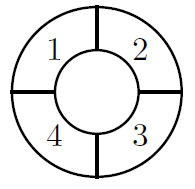
\includegraphics[scale=1]{clase_05_dona.png}
\end{center}
Vamos a separar el problema en dos casos:

\begin{enumerate}
    \item Si las casas 1 y 3 tienen el mismo color, hay cuatro maneras de elegir ese color. Podemos elegir el color de la casa 2 de tres maneras (simplemente no puede ser el color usado en las casas 1 y 3), lo mismo ocurre para la casa 4. Por lo tanto, hay $4 \times 3 \times 3 = 36$ maneras de pintar de esta forma.
    \item Ahora, si 1 y 3 tienen colores diferentes, podemos elegir el color de la casa 1 de cuatro maneras, el de la casa 3 de tres maneras y, de las casas 2 y 4, podemos elegir de dos maneras cada una. Así que hay $4 \times 3 \times 2 \times 2 = 48$ maneras de pintar de esta otra forma.
\end{enumerate}

Por lo tanto, podemos concluir que hay $36 + 48 = 84$ maneras de pintar la rosquilla.

\begin{example}
¿Cuántos son los números de cuatro dígitos que no tienen dos dígitos consecutivos con la misma paridad?
\end{example}

Vamos a separar el problema en dos casos:

\begin{enumerate}
    \item Cuando el primer dígito es par, hay 4 posibilidades para el primer dígito, 5 para el segundo, 5 para el tercero y 5 para el último. Totalizando $4 \times 5 \times 5 \times 5 = 500$ números.
    \item Cuando el primer dígito es impar, hay 5 posibilidades para cada uno de los dígitos. Por lo tanto, la cantidad de números de esta forma es $5 \times 5 \times 5 \times 5 = 625$.
\end{enumerate}

Por lo tanto, hay un total de $625 + 500 = 1125$ números de cuatro dígitos que no tienen dos dígitos consecutivos con la misma paridad.

\section*{Conteos Múltiples}

Los problemas que hemos abordado hasta ahora tenían algo en común: el papel de la ordenación en la diferenciación de las posibilidades. Sin embargo, hay casos en los que el orden de los elementos no es relevante para el conteo.

\begin{claim}[Situación 1]
De un grupo de 7 personas, debemos elegir 3 de ellas para formar un podio (primer, segundo y tercer lugares). ¿De cuántas formas podemos hacerlo?
\end{claim}

\begin{claim}[Situación 2]
    De un grupo de 7 personas, debemos elegir 3 de ellas para formar un comité (sin jerarquías). ¿De cuántas formas podemos hacerlo?
\end{claim}

Es importante notar que, aunque son similares, son problemas diferentes, con respuestas también diferentes. Sabemos cómo resolver el primero. La respuesta es $7 \times 6 \times 5 = 210$. Ahora, sabiendo esta respuesta, podemos dar una solución para el segundo problema.

Observa que, para cada comité formado, podemos construir $3 \times 2 \times 1 = 6$ podios distintos. Por lo tanto, el número de podios es seis veces el número de comités. Así que la respuesta para el segundo problema es

\[
\frac{210}{6} = 35.
\]

Podemos usar esta estrategia para resolver problemas de anagramas en los que las palabras tienen letras repetidas.

\begin{example}
¿Cuántos anagramas\footnote[1]{Un anagrama es una palabra o frase que se obtiene al reordenar las letras de otra palabra o frase. Por ejemplo, un anagrama de la palabra ``letras'' sería ``lastre'' y el anagrama de ``frase'' sería ``fresa''.} tiene la palabra matemática (sin tener en cuenta los acentos)?
\end{example}

Si imaginamos por un momento una palabra de 10 letras diferentes:

\[
m_1a_1t_1e_1m_2a_2t_2i_1c_1a_3,
\]

el número total de anagramas será $10!$. Sin embargo, al intercambiar letras que en realidad son iguales (como $a_1$ y $a_3$), el anagrama sigue siendo el mismo. Por lo tanto, cada anagrama ha sido contado $2 \times 2 \times 3!$ veces. Por lo tanto, la respuesta es

\[
\frac{10!}{2 \times 2 \times 3!}.
\]

\begin{example}
¿De cuántas formas podemos poner ocho personas en una fila si Alice y Bob deben estar juntos, y Carol debe estar en algún lugar detrás de Daniel?
\end{example}

Vamos a imaginar a Alice y Bob como una única persona. Habrá $7! = 5040$ posibilidades. Alice puede estar delante de Bob o viceversa. Entonces debemos multiplicar el número de posibilidades por 2. Por otro lado, Carol está detrás de Daniel en exactamente la mitad de estas permutaciones, así que la respuesta es simplemente 5040.

\Opensolutionfile{all-hints}

\section{Problemas Propuestos}
\begin{problem}
Se escriben todos los enteros del 1 al 9999. ¿Cuántos números tienen al menos un cero?
\begin{hint}
Encuentra la cantidad de números del 0 al 9999 que no contienen ningún dígito cero. Haz esta cuenta separándola en cuatro casos (de acuerdo con la cantidad de dígitos).\\

Contemos cuántos no tienen ningún dígito cero. Del 1 al 9 tenemos 9 dígitos sin ningún cero. De 10 a 99, tenemos $9 \times 9 = 81$ números sin ningún cero. De 100 a 999 tenemos $9 \times 9 \times 9 = 729$ números sin ningún cero. De 1000 a 9999 tenemos $9^4 = 6561$ números sin ningún cero. Por lo tanto, entre 1 y 9999 tenemos $9 + 81 + 729 + 6561 = 7380$ números sin ningún cero. Por lo tanto, hay $9999 - 7380 = 2619$ números con al menos un cero.
\end{hint}
\end{problem}

\begin{problem}
¿Cuántos números de tres dígitos tienen todos sus dígitos con la misma paridad?
\begin{hint}
Separa en dos casos:\begin{itemize}
\item[1)] cuando todos los dígitos son pares;
\item[2)] cuando todos los dígitos son impares. ¡No olvides que cero no puede ser el primer dígito!
\end{itemize}

Si todos los dígitos son pares, tenemos $4 \times 5 \times 5 = 100$ números, recordando que el primer dígito no puede ser cero. Si todos los dígitos son impares, tenemos $5^3 = 125$ números. Por lo tanto, el total es $100 + 125 = 225$.

\end{hint}
\end{problem}

\begin{problem}
¿Cuántos son los números de cuatro dígitos que tienen al menos un dígito repetido?
\begin{hint}
Hay $9 \times 9 \times 8 \times 7 = 4536$ números de cuatro dígitos con todos los dígitos distintos. Como hay en total 9000 números de cuatro dígitos, tenemos $9000 - 4536 = 4464$ números con al menos un dígito repetido.\\

Hay $9 \times 9 \times 8 \times 7 = 4536$ números de cuatro dígitos con todos los dígitos distintos. Como hay en total 9000 números de cuatro dígitos, tenemos $9000 - 4536 = 4464$ números con al menos un dígito repetido.
\end{hint}
\end{problem}

\begin{problem}
¿Cuántos son los números de cuatro dígitos distintos que no tienen dos dígitos consecutivos con la misma paridad?
\begin{hint}
Consideremos el número de representación decimal $abcd$. Entonces, inicialmente tenemos 9 opciones para $a$. Una vez elegido $a$, sabemos que $b$ debe tener paridad diferente, por lo que tiene 5 opciones. El dígito $c$ debe tener la misma paridad que $a$ y no puede ser igual a él, por lo que solo tiene 4 opciones. El dígito $d$ debe tener la misma paridad que $c$ y debe ser diferente de él, por lo que tiene 4 opciones. La cantidad total de números que satisfacen las condiciones del enunciado es $9 \times 5 \times 4 \times 4 = 720$.\\

Consideremos el número de representación decimal $abcd$. Entonces, inicialmente tenemos 9 opciones para $a$. Una vez elegido $a$, sabemos que $b$ debe tener paridad diferente, por lo que tiene 5 opciones. El dígito $c$ debe tener la misma paridad que $a$ y no puede ser igual a él, por lo que solo tiene 4 opciones. El dígito $d$ debe tener la misma paridad que $c$ y debe ser diferente de él, por lo que tiene 4 opciones. La cantidad total de números que satisfacen las condiciones del enunciado es $9 \times 5 \times 4 \times 4 = 720$.
\end{hint}
\end{problem}

\begin{problem}
¿De cuántas maneras podemos colocar un rey negro y un rey blanco en un tablero de ajedrez (\(8 \times 8\)) sin que ninguno de ellos se ataque?
\begin{hint}
Podemos dividir el tablero en tres regiones: la primera está formada por las cuatro casillas en las esquinas del tablero; la segunda por las 24 casillas del borde (que no están en las esquinas); y la tercera por el tablero 6 × 6 en el interior del tablero. Si el primer rey se coloca en la primera región, hay 60 formas de colocar el segundo rey; si se coloca en la segunda, hay 58 formas; y si se coloca en la tercera, hay 55 formas. Por lo tanto, tenemos un total de $4 \times 60 + 24 \times 58 + 36 \times 55 = 3612$ modos diferentes de colocar los dos reyes.\\

Podemos dividir el tablero en tres regiones: la primera está formada por las cuatro casillas en las esquinas del tablero; la segunda por las 24 casillas del borde (que no están en las esquinas); y la tercera por el tablero 6 × 6 en el interior del tablero. Si el primer rey se coloca en la primera región, hay 60 maneras de colocar el segundo rey; si se coloca en la segunda, hay 58 maneras; y si se coloca en la tercera, hay 55 maneras. Por lo tanto, tenemos un total de $4 \times 60 + 24 \times 58 + 36 \times 55 = 3612$ modos diferentes de colocar los dos reyes.
\end{hint}
\end{problem}

\begin{problem}
¿Cuántos son los números naturales pares que se escriben con tres dígitos distintos?
\begin{hint}
Consideremos el número $abc$. Vamos a separar el problema en 3 casos.\begin{itemize}
\item $c = 0$: $a$ puede asumir 9 valores y $b$ solamente 8, ya que no puede ser igual a ningún otro;
\item $b = 0$: $c$ puede asumir 4 valores, ya que es par, y así $a$ podrá asumir 8 valores;
\item $b, c \neq 0$: $c$ puede asumir 4 valores, por lo tanto $a$ puede tener 8 valores, así \(b\) podrá tomar 7 valores.
\end{itemize}
Luego, tenemos \(9\cdot 8 + 4\cdot 8 + 4\cdot 8\cdot 7 = 328\) números.
\end{hint}
\end{problem}

\begin{problem}
En la ciudad Gótica, las placas de las motos consisten en tres letras. La primera letra debe estar en el conjunto \{C, H, L, P, R\}, la segunda letra en el conjunto \{A, I, O\}, y la tercera letra en el conjunto \{D, M, N, T\}. Un día, se decidió aumentar el número de placas usando dos nuevas letras J y K. El intendente de transportes ordenó que las nuevas letras se colocaran en conjuntos diferentes. Determine con qué opción podemos obtener el mayor número de placas.
\begin{hint}
Inicialmente tenemos $5 \times 3 \times 4 = 60$ placas. De acuerdo con el problema, tenemos las siguientes opciones para el nuevo número de placas: $6 \times 4 \times 4 = 96$, $5 \times 4 \times 5 = 100$ y $6 \times 3 \times 5 = 90$. Por lo tanto, el número máximo es 100.
\end{hint}
\end{problem}

\begin{problem}[Mayo de 1998] Cada uno de los seis segmentos de la figura a continuación debe ser pintado de una de cuatro colores de modo que los segmentos adyacentes no tengan el mismo color. ¿De cuántas maneras podemos hacer esto?
\begin{center}
    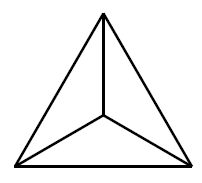
\includegraphics[scale=1]{images/clase_05_mayo.png}
\end{center}
\begin{hint}
Hay $4 \times 3 \times 2 = 24$ formas de pintar el triángulo externo. Observa que el cuarto color (el que no se usó en el triángulo) debe aparecer ninguna o una vez en los tres segmentos internos. Si aparece más de una vez, habrá dos segmentos adyacentes con el mismo color. Por lo tanto, tenemos dos casos:
\begin{itemize}
\item Si el cuarto color no aparece ninguna vez, entonces solo hay una forma de pintar los segmentos internos, con cada segmento teniendo el mismo color que el lado opuesto del triángulo mayor.
\item Si el cuarto color aparece una vez, puede aparecer en cualquiera de los tres segmentos internos. Una vez que se elige el segmento que tendrá el cuarto color, los otros colores quedan definidos. Por lo tanto, hay 3 pinturas diferentes.
\end{itemize}
El número de formas de pintar la figura es $24 \times (1 + 3) = 96$. Si consideramos las rotaciones de la figura, solo hay $\frac{96}{3} = 32$ pinturas diferentes.
\end{hint}
\end{problem}

\begin{problem}
En una fiesta había 6 hombres y 4 mujeres. ¿De cuántas maneras podemos formar 3 parejas con estas personas?
\begin{hint}
\[ \frac{(6 \times 5 \times 4) \times (4 \times 3 \times 2)}{3!}.\]
Tenemos $6 \times 4$ formas de elegir la primera pareja. Para la segunda pareja, tenemos $5 \times 3$ y para la tercera pareja, $4 \times 2$. Sin embargo, el orden en que elegimos las parejas no importa. Por lo tanto, debemos dividir el resultado por $3!$.

Así, la respuesta es:

$$
\frac{(6 \times 4) \times (5 \times 3) \times (4 \times 2)}{3!} = 480.
$$
\end{hint}
\end{problem}

\begin{problem}
¿De cuántas maneras podemos poner tres torres del mismo color en un tablero \(8 \times 8\) de modo que ninguna de ellas se ataque?
\begin{hint}
\[\frac{64 \times 49 \times 36}{3!}.\]
Para la primera torre, tenemos 64 casillas disponibles, para la segunda tenemos 49 casillas y para la tercera tenemos 36 casillas. Sin embargo, como el orden de colocación de las torres no importa, debemos dividir por $3!$.

El resultado es:

$$
\frac{64 \times 49 \times 36}{3!} = 18816.
$$
\end{hint}
\end{problem}

\begin{problem}[AIME 1996] Dos casillas de un tablero \(7\times 7\) están pintadas de amarillo y las demás están pintadas de verde. Dos pinturas se consideran equivalentes si una se obtiene de la otra mediante una rotación aplicada en el plano del tablero. ¿Cuántas pinturas inequivalentes existen?
\begin{hint}
Separa el problema en dos casos. Cuando las casillas amarillas son simétricas con respecto al centro del tablero y cuando no lo son. Cuenta el número de pinturas equivalentes en cada caso.\\
Vamos a dividir el problema en dos casos.

\begin{enumerate}
    \item \textbf{Caso 1:} Supongamos que las dos casas amarillas son simétricas respecto al centro. Escogiendo una casa, la otra queda determinada. Hay $48$ formas de elegir la primera casa (no puede ser la central) y $1$ de elegir la segunda. Como el orden de elección de las casas no importa, debemos dividir el resultado por $2!$. Sin embargo, como las casas son simétricas respecto al centro, obtenemos $2$ configuraciones diferentes. Por lo tanto, debemos dividir el resultado nuevamente por $2$. El número de pinturas inequivalentes en este caso es:
    \[
    \frac{48}{2! \times 2} = 12.
    \]
    
    \item \textbf{Caso 2:} Supongamos que las dos casas no son simétricas respecto al centro y ninguna de las dos es la casa central. Hay $48$ formas de elegir la primera casa y $46$ formas de elegir la segunda casa (no puede ser igual a la primera ni a su simétrica, ni puede ser la central). Como el orden de elección no importa y la rotación genera $4$ configuraciones diferentes, debemos dividir el resultado por $2! \times 4$. El número de pinturas inequivalentes en este caso es:
    \[
    \frac{48 \times 46}{2! \times 4} = 276.
    \]
    
    \item \textbf{Caso 3:} Supongamos que una de las casas está en el centro. El número de formas de obtener esto es $48$. Rotando el tablero, obtenemos $4$ configuraciones distintas. Por lo tanto, el número de pinturas inequivalentes en este caso es:
    \[
    \frac{48}{4} = 12.
    \]
\end{enumerate}

El número total de pinturas inequivalentes es $12 + 276 + 12 = 300$.
\end{hint}
\end{problem}

\begin{problem}
En un salón de clases hay a niñas y b niños. ¿De cuántas formas pueden colocarse en una fila, si las niñas deben estar en orden creciente de peso, y los niños también? (Suponga que ninguna 2 personas tienen el mismo peso).
\begin{hint}
Tenemos $(a + b)!$ maneras de permutar a todos los niños. Sin embargo, solo una de las $a!$ permutaciones de las niñas está en el orden correcto y solo $b!$ de las permutaciones de los niños están en el orden correcto. Por lo tanto, la respuesta es

\[
\frac{(a + b)!}{a!b!}.
\]

\end{hint}
\end{problem}

\begin{problem}
Considere un torneo de ajedrez con 10 participantes. En la primera ronda cada participante juega solo una vez, de modo que hay 5 juegos realizados simultáneamente. ¿De cuántas maneras puede realizarse esta primera ronda?
\begin{hint}
.
\end{hint}
\end{problem}

\begin{problem}
Doce caballeros están sentados alrededor de una mesa redonda. Cada uno de los 12 caballeros considera a sus dos vecinos como rivales. Se desea formar un grupo de 5 caballeros para salvar a una princesa. En este grupo no puede haber caballeros rivales. Determine de cuántas maneras es posible elegir este grupo.
\begin{hint}
..
\end{hint}
\end{problem}

\Closesolutionfile{all-hints}

\section{Sugerencias y Soluciones}
\begin{enumerate}
\input{all-hints.out}
\end{enumerate}

\end{document}